\documentclass[border=3mm,
               tikz,
               preview,
               dvipsnames,
               ]{standalone}
\usepackage{pgfplots}
\usepackage{siunitx}
\pgfplotsset{width=8cm,compat=newest}
\usepackage{pgfplotstable}


\begin{document}
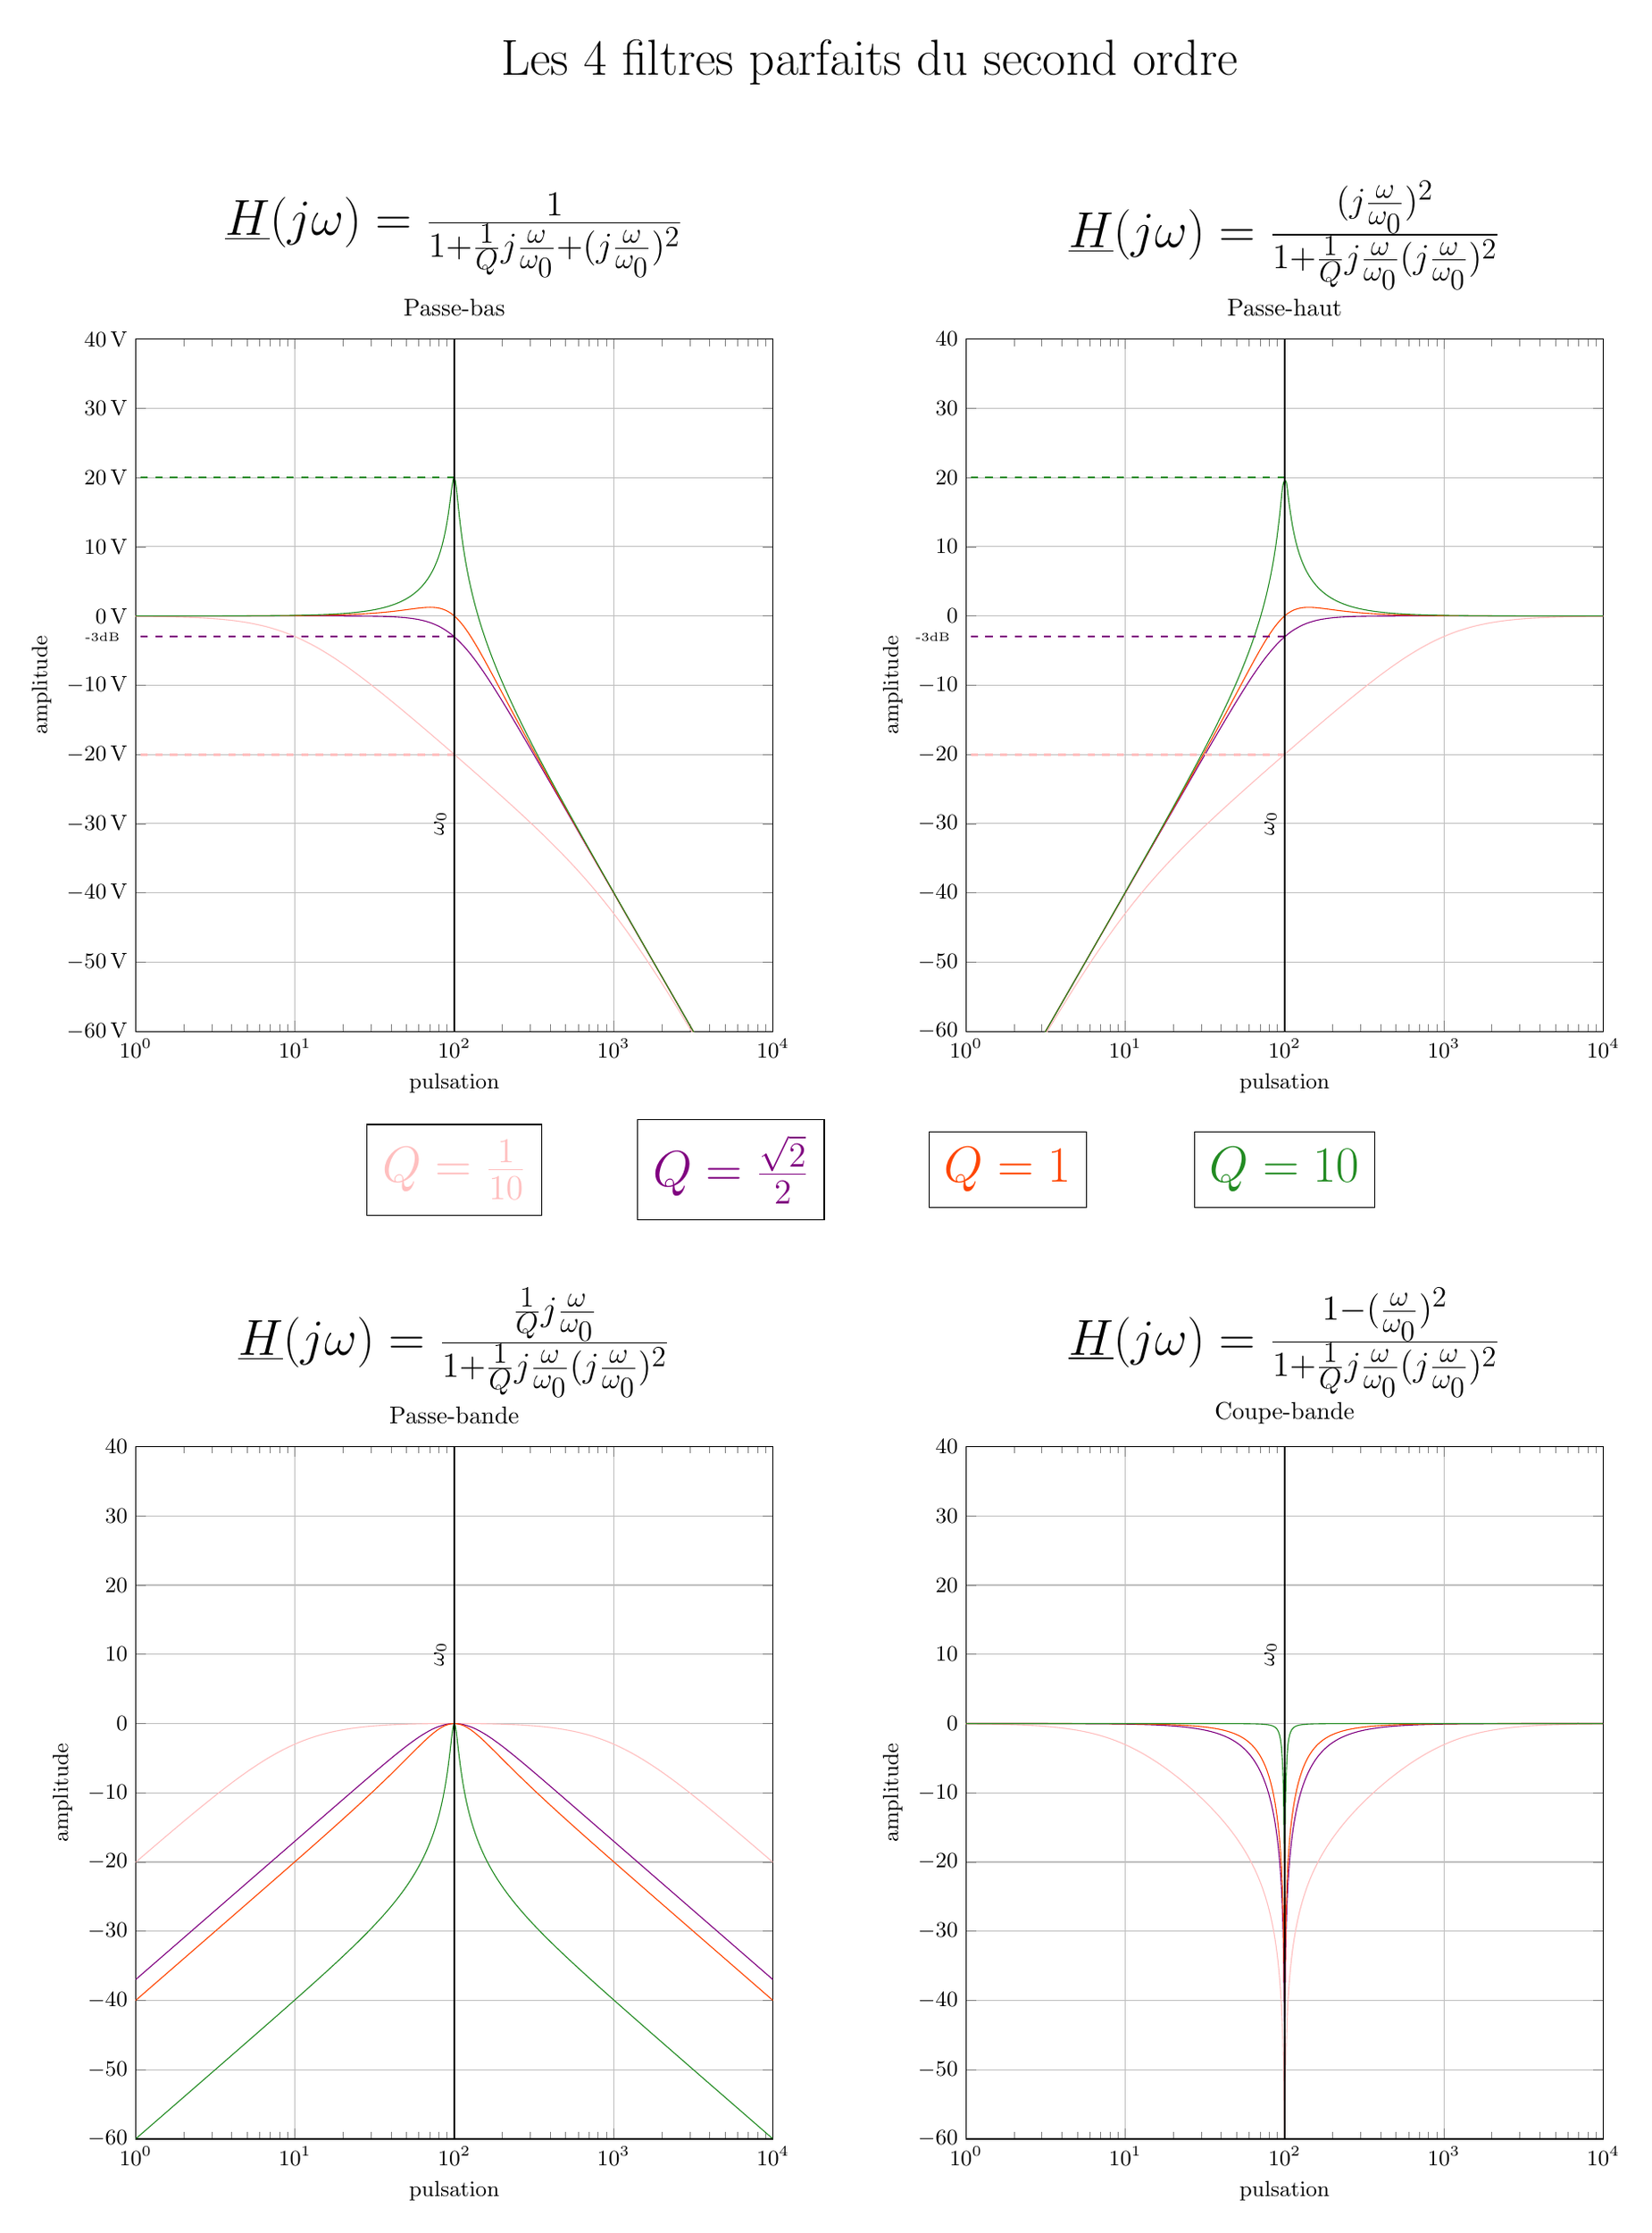
\begin{tikzpicture}
\huge
\node[align=center] at (0,23) {Les 4 filtres parfaits du second ordre};
\node[draw,align=center,text=pink] at (-6,7) {$Q=\frac{1}{10}$};
\node[draw,align=center,text=violet] at (-2,7) {$Q=\frac{\sqrt{2}}{2}$};
\node[draw,align=center,text=OrangeRed] at (2,7) {$Q=1$};
\node[draw,align=center,text=ForestGreen] at (6,7) {$Q=10$};
\huge

\node[align=center,text=black] at (-6,20.5) {$\underline{H}(j\omega)=\frac{1}{1+\frac{1}{Q}j\frac{\omega}{\omega_0}+(j\frac{\omega}{\omega_0})^2}$};
\node[align=center,text=black] at (6,20.5) {$\underline{H}(j\omega)=\frac{(j\frac{\omega}{\omega_0})^2}{1+\frac{1}{Q}j\frac{\omega}{\omega_0}(j\frac{\omega}{\omega_0})^2}$};
\node[align=center,text=black] at (-6,4.5) {$\underline{H}(j\omega)=\frac{\frac{1}{Q}j\frac{\omega}{\omega_0}}{1+\frac{1}{Q}j\frac{\omega}{\omega_0}(j\frac{\omega}{\omega_0})^2}$};
\node[align=center,text=black] at (6,4.5) {$\underline{H}(j\omega)=\frac{1-(\frac{\omega}{\omega_0})^2}{1+\frac{1}{Q}j\frac{\omega}{\omega_0}(j\frac{\omega}{\omega_0})^2}$};
\small
\coordinate (Pbas) at (-6,14);
\coordinate (Phaut) at (6,14);
\coordinate (Pbande) at (-6,-2);
\coordinate (Cbande) at (6,-2);
\begin{semilogxaxis}[
at=(Pbas),	
anchor=center,
title={\normalsize Passe-bas},
xlabel={pulsation},
ylabel={amplitude},
grid=major,
smooth,
xmax=10^4,
xmin=1,
ymin=-60,
ymax=40,
x=1cm,
y=0.1cm,
yticklabel={\SI[round-mode=places, round-precision=0]{\tick}{V}}
]

\addplot[samples=40,domain=1:10000,color=pink]{
-10*log10((x/10)^2 + (1-x^2/100^2)^2)
};
\addplot[samples=100,domain=1:10000,color=violet]{
-10*log10((x/100*sqrt(2))^2 + (1-x^2/100^2)^2)
};
\addplot[samples=200,domain=1:10000,color=OrangeRed]{
-10*log10((x/100)^2 + (1-x^2/100^2)^2)
};
\addplot[samples=500,domain=1:10000,color=ForestGreen]{
-10*log10((x/1000)^2 + (1-x^2/100^2)^2)
};
\coordinate (20DB0) at (axis cs:1,20);
\coordinate (20DB100) at (axis cs:100,20);
\draw[dashed,color=ForestGreen,line width = 0.3mm] (20DB100) -- (20DB0);
\coordinate (-3DB0) at (axis cs:1,-3);
\coordinate (-3DB100) at (axis cs:100,-3);
\draw[dashed,color=violet, line width = 0.2mm] (-3DB100) -- (-3DB0);
\coordinate (-20DB0) at (axis cs:1,-20);
\coordinate (-20DB100) at (axis cs:100,-20);
\draw[dashed,color=pink, line width = 0.4mm] (-20DB100) -- (-20DB0);
\draw[color=black,line width=0.2mm](axis cs:100,-60) -- (axis cs:100,40) node[pos=0.3,rotate=90,above] {$\omega_0$};
\end{semilogxaxis}
\node[label=left:\tiny -3dB] at (-3DB0) {};
\begin{semilogxaxis}[
at=(Phaut),
anchor=center,
title={\normalsize Passe-haut},,
xlabel={pulsation},
ylabel={amplitude},
grid=major,
smooth,
xmax=10^4,
xmin=1,
ymin=-60,
ymax=40,
x=1cm,
y=0.1cm]
\addplot[samples=40,domain=1:10000,color=pink]{
10*log10( (x^2/10000)^2 / ((x/10)^2 + (1-x^2/100^2)^2) )
};
\addplot[samples=50,domain=1:10000,color=violet]{
10*log10((x^2/10000)^2/((x/100*sqrt(2))^2 + (1-x^2/100^2)^2))
};
\addplot[samples=100,domain=1:10000,color=OrangeRed]{
10*log10((x^2/10000)^2/((x/100)^2 + (1-x^2/100^2)^2))
};
\addplot[samples=200,domain=1:10000,color=ForestGreen]{
10*log10((x^2/10000)^2/((x/1000)^2 + (1-x^2/100^2)^2))
};
\coordinate (20DB0) at (axis cs:1,20);
\coordinate (20DB100) at (axis cs:100,20);
\draw[dashed,color=ForestGreen,line width = 0.3mm] (20DB100) -- (20DB0);
\coordinate (-3DB0) at (axis cs:1,-3);
\coordinate (-3DB100) at (axis cs:100,-3);
\draw[dashed,color=violet, line width = 0.2mm] (-3DB100) -- (-3DB0);
\coordinate (-20DB0) at (axis cs:1,-20);
\coordinate (-20DB100) at (axis cs:100,-20);
\draw[dashed,color=pink, line width = 0.4mm] (-20DB100) -- (-20DB0);
\draw[color=black,line width=0.2mm](axis cs:100,-60) -- (axis cs:100,40) node[pos=0.3,rotate=90,above] {$\omega_0$};
\end{semilogxaxis}
\node[label=left:\tiny -3dB] at (-3DB0) {};
\begin{semilogxaxis}[
at=(Pbande),
anchor=center,
title={\normalsize Passe-bande},,
xlabel={pulsation},
ylabel={amplitude},
grid=major,
smooth,
xmax=10^4,
xmin=1,
ymin=-60,
ymax=40,
x=1cm,
y=0.1cm]
\addplot[samples=40,domain=1:10000,color=pink]{
10*log10((10*x/100)^2/((x/10)^2 + (1-x^2/100^2)^2))
};
\addplot[samples=50,domain=1:10000,color=violet]{
10*log10((x/100*sqrt(2))^2/((x/100*sqrt(2))^2 + (1-x^2/100^2)^2))
};
\addplot[samples=100,domain=1:10000,color=OrangeRed]{
10*log10((x/100)^2/((x/100)^2 + (1-x^2/100^2)^2))
};
\addplot[samples=800,domain=1:10000,color=ForestGreen]{
10*log10((0.1*x/100)^2/((x/1000)^2 + (1-x^2/100^2)^2))
};
\draw[color=black,line width=0.2mm](axis cs:100,-60) -- (axis cs:100,40) node[pos=0.7,rotate=90,above] {$\omega_0$};
\end{semilogxaxis}

\begin{semilogxaxis}[
at=(Cbande),
anchor=center,
title={\normalsize Coupe-bande},
xlabel={pulsation},
ylabel={amplitude},
grid=major,
smooth,
xmax=10^4,
xmin=1,
ymin=-60,
ymax=40,
x=1cm,
y=0.1cm]
\addplot[samples=1000,domain=1:10000,color=pink]{
10*log10((1-x^2/10000)^2/((x/10)^2 + (1-x^2/100^2)^2))
};
\addplot[samples=1000,domain=1:10000,color=violet]{
10*log10((1-x^2/10000)^2/((x/100*sqrt(2))^2 + (1-x^2/100^2)^2))
};
\addplot[samples=1000,domain=1:10000,color=OrangeRed]{
10*log10((1-x^2/10000)^2/((x/100)^2 + (1-x^2/100^2)^2))
};
\addplot[samples=1000,domain=1:10000,color=ForestGreen]{
10*log10((1-x^2/10000)^2/((x/1000)^2 + (1-x^2/100^2)^2))
};
\draw[color=black,line width=0.2mm](axis cs:100,-60) -- (axis cs:100,40) node[pos=0.7,rotate=90,above] {$\omega_0$};
\end{semilogxaxis}
\end{tikzpicture}



\end{document}